\documentclass{beamer}

% Size of poster
\usepackage[size=a0,orientation=portrait]{beamerposter}

% Theme and color  https://hartwork.org/beamer-theme-matrix/
\usetheme{Berlin}
\usecolortheme{beaver}

% Packages
\usepackage{lipsum}      % Use for dummy text, for instance \lipsum[1-4] prints 4 paragraphs

\usepackage[english]{babel}
\usepackage[latin1]{inputenc}
\usepackage{multicol}
\usepackage{multirow}
\usepackage{tabularx}
%\newcolumntype{C}{>{\centering\arraybackslash}X}

%\usepackage{amsmath,amsthm, amssymb, latexsym}
%\boldmath

% Environment with extra margins  https://tex.stackexchange.com/a/108495
\newenvironment<>{Block}[1]{%
 \begin{actionenv}#2%
 \def\insertblocktitle{\leftskip=10pt\rightskip=10pt\vspace*{-3pt} #1\vspace{10pt}}%
 \par%
 \usebeamertemplate{block begin}\leftskip=10pt\rightskip=10pt\vspace{10pt}}
 {\par\vspace{10pt}\usebeamertemplate{block end}
 \end{actionenv}}

\addtobeamertemplate{block begin}{}{\setlength{\parskip}{20pt plus 1pt minus 1pt}}
\setbeamertemplate{caption}[numbered]

% Bibliography colors and labels
\setbeamertemplate{bibliography item}{\color{black}\insertbiblabel}
\setbeamercolor{bibliography entry item}{fg=black}
\setbeamercolor{bibliography entry author}{fg=black}
\setbeamercolor{bibliography entry title}{fg=black} 
\setbeamercolor{bibliography entry location}{fg=black} 
\setbeamercolor{bibliography entry note}{fg=black}

\usebackgroundtemplate{\includegraphics[width=\paperwidth]{figure/header}}

\begin{document}
\begin{frame}[t]
  % Top Header is on background
  \vspace*{20cm}

  % Line with author information
  \begin{columns}
    \begin{column}[t]{.10\textwidth} %spacer
    \end{column}
    \begin{column}[t]{.35\textwidth}
      {\begin{flushright}
          \fontsize{42}{48}\selectfont Geir Arne Hjelle\\
          \fontsize{24}{24}\selectfont \texttt{geir.arne.hjelle@kartverket.no}\\
          \fontsize{24}{24}\selectfont {\itshape Norwegian Mapping Authority}
      \end{flushright}}
    \end{column}
    \begin{column}[t]{.35\textwidth}
      {\begin{flushleft}
          \fontsize{42}{48}\selectfont Kristian Evers\\
          \fontsize{24}{24}\selectfont \texttt{kreve@sdfe.dk}\\
          \fontsize{24}{24}\selectfont {\itshape Danish Agency for Data Supply and Efficiency}
      \end{flushleft}}
    \end{column}
    \begin{column}[t]{.10\textwidth} %spacer
    \end{column}
  \end{columns}

  \vspace*{2cm}

  % Content area

  \begin{columns}
    \begin{column}[t]{.98\textwidth}
      \begin{Block}{Background}
        \begin{multicols}{4}
          In geodesy we often deal with lists of coordinates and/or velocities of ground
markers and GNSS stations. These lists come in many shapes and sizes. Often the
points are represented in text files in a structured format but they can just as
easily be presented as a binary file in various formats. The files can be
generated by widely used software such as Bernese or perhaps by software only
meant for internal use in a national geodetic office.

An example of the latter is the KMS-format used in Denmark. KMS files come as
unstructured text files that are particularly difficult to parse by standard
text import tools. Similarly much work in Norway is based on the SOSI and FRI
formats. Converting between various file formats is often challenging making
data exchange from one software to another difficult.

One possible solution would be a standard file format for exchange of geodetic
data. Currently no definitive standard file format for exchange of coordinates
and velocities has been agreed upon in the geodetic community. While such a
format would indeed be nice to have, it is near impossible to get to a stage
where a single format is agreed as the work to implement it everywhere would be
immense.

Instead, we propose a new software that seamlessly converts between all common
formats. The inspiration to this approach comes from tools such as GDAL and
PDAL used in the world of remote sensing with great success. The new software
for converting between geodetic file formats has been named \textbf{Posetta},
obviously a play on words, in that this is a sort of Rosetta Stone for
positions.

%% Posetta is a NKG collaboration that so far only exists as a prototype. At the
%% time of writing Posetta can only convert between a few different file formats
%% but the architectural foundation has been created and adding new file formats is
%% fairly easy. We hope this tool will become useful for all geodesist within the
%% NKG and eliminate the need for reformatting files manually in the future.

\endinput

        \end{multicols}
      \end{Block}
    \end{column}
  \end{columns}

  \vspace*{2cm}     % Some space before Figures

  % Figure strip
  \begin{columns}
    \begin{column}[b]{.24\textwidth}
      \begin{figure}
        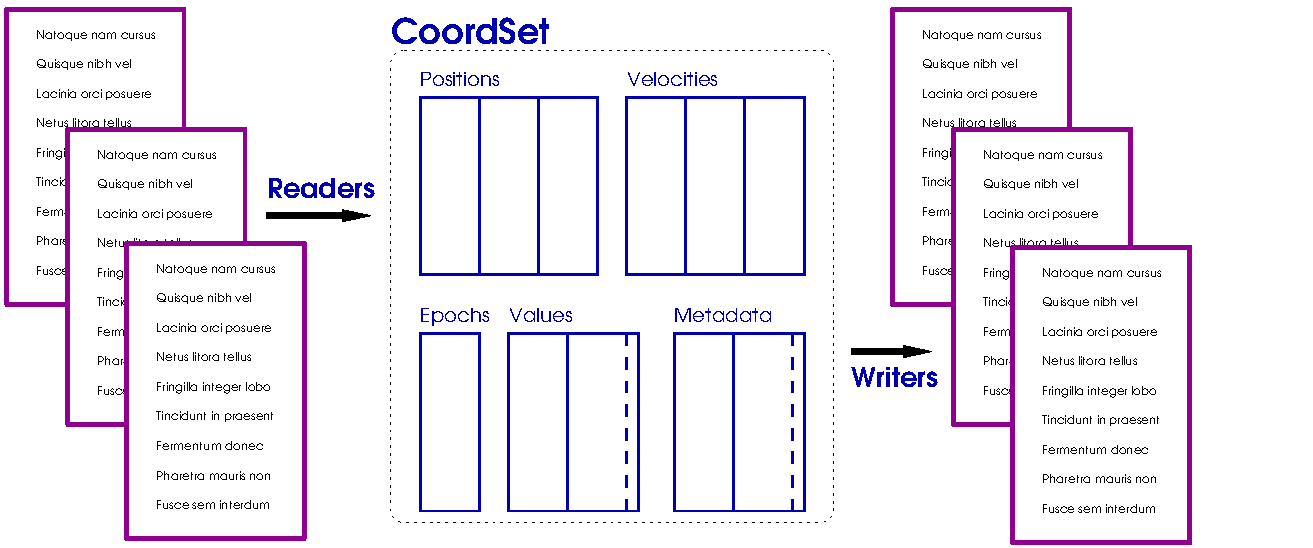
\includegraphics[width=\textwidth]{figure/coordset}
        \caption{The \texttt{CoordSet} is the internal representation of coordinates}
        \label{fig:coordset}
      \end{figure}
    \end{column}

    \begin{column}[b]{.24\textwidth}
      \begin{figure}
        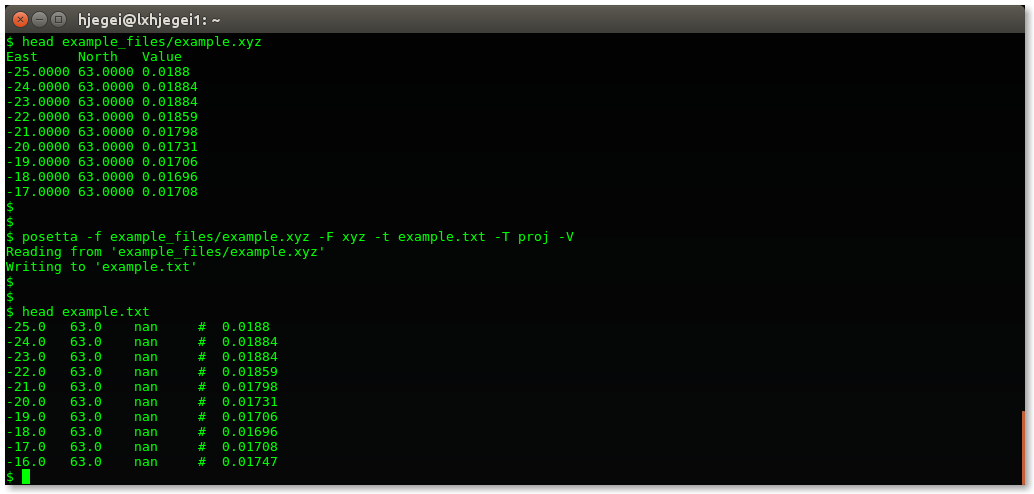
\includegraphics[width=\textwidth]{figure/posetta_cli}
        \caption{Using Posetta as a command line program}
        \label{fig:cli}
      \end{figure}
    \end{column}

    \begin{column}[b]{.24\textwidth}
      \begin{figure}
        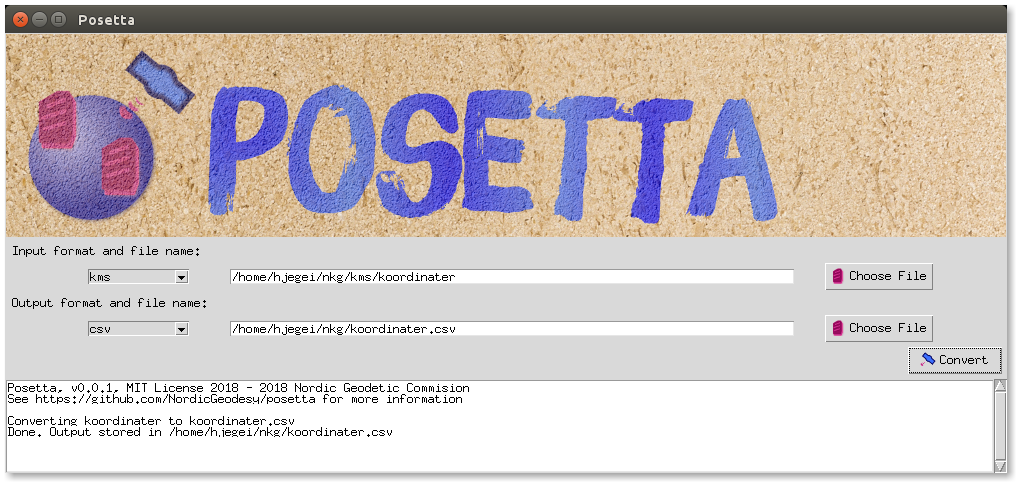
\includegraphics[width=\textwidth]{figure/posetta_gui}
        \caption{The graphical user interface of Posetta}
        \label{fig:gui}
      \end{figure}
    \end{column}

    \begin{column}[b]{.24\textwidth}
      \begin{figure}
        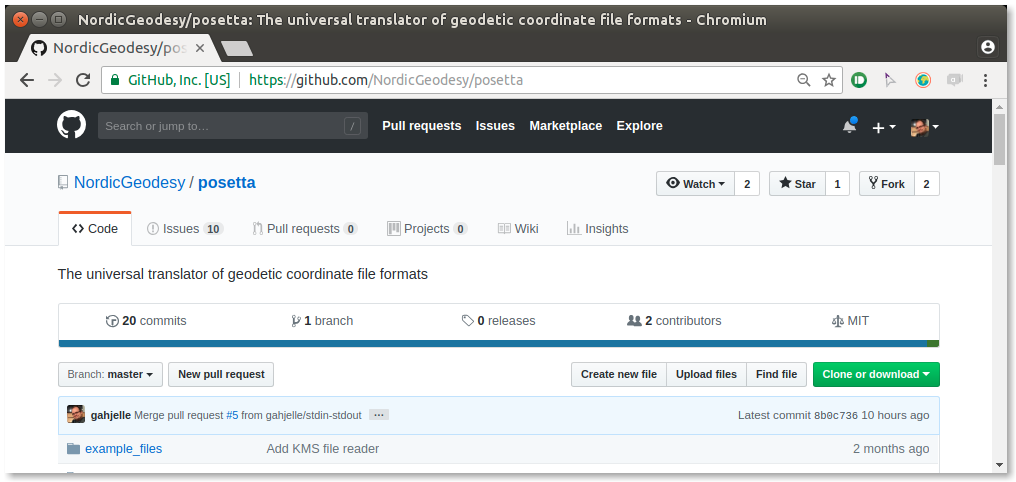
\includegraphics[width=\textwidth]{figure/posetta_github}
        \caption{You can download or contribute to Posetta at Github}
        \label{fig:github}
      \end{figure}
    \end{column}
  \end{columns}

  \vspace*{2cm}

  \begin{columns}
    \begin{column}[t]{.98\textwidth}
      \begin{Block}{Technology}
        \begin{multicols}{4}
          Posetta is written in Python. It is supported on Windows, MacOS, and Linux running Python 3.6 or later. Posetta can be used either as a command line program (see Figure~\ref{fig:cli}) or through a graphical user interface (see Figure~\ref{fig:gui}).

\columnbreak
Posetta has a fairly simple architecture, built around something we call a \texttt{CoordSet}. The \texttt{CoordSet} is a class that represents a set of coordinates, either as a list of points or as a grid (see Figure~\ref{fig:coordset}. The \texttt{CoordSet} consists of tables with information about the position, velocity, epoch, measurement values, and other metadata for each point.

Furthermore:

\begin{itemize}
\item Posetta has \textbf{readers}. Each reader can read one format and convert it to a \texttt{CoordSet}.
\item Posetta has \textbf{writers}. Each writer can convert a \texttt{CoordSet} to a format and write it to file.
\end{itemize}

Using these readers and writers, we can convert from any supported input format to any supported output format.

The \texttt{CoordSet} can also easily be converted to \texttt{numpy} arrays~\cite{oliphant2006} or \texttt{pandas} dataframes~\cite{mckinney2010}. This means that you can also take advantage of Posetta's readers and writers inside your own Python programs.

\endinput

        \end{multicols}
      \end{Block}
    \end{column}
  \end{columns}

  \vspace*{2cm}

  \begin{columns}
    \begin{column}[t]{.48\textwidth}
      \begin{Block}{Input and Output Formats}
        At the moment only a few formats have been implemented (indicated in \textbf{bold} below). However the plan is to add all the formats in common use within the NKG.  Please let us know if you use any formats not listed. Either write its name below, or post an issue or contribute code at \texttt{github.com/nordicgeodesy/posetta}.

\begin{multicols}{2}
  \textbf{Input Formats}
  
  \begin{itemize}
  \item BIN - Binary grid format
  \item \textbf{CSV} - General comma separated text format
  \item FRI - Norwegian free form text format
  \item GRI - Text grid format (BIN companion)
  \item \textbf{KMS} - Danish coordinate format
  \item \textbf{PROJ} - Column based text format
  \item SOSI - Norwegian geodata format
  \item Where Dataset
  \item \textbf{XYZ} - Three column text format
  \end{itemize}

  \columnbreak
  \textbf{Output Formats}
  
  \begin{itemize}
  \item BIN - Binary grid format
  \item \textbf{CSV} - General comma separated text format
  \item FRI - Norwegian free form text format
  \item GRI - Text grid format (BIN companion)
  \item KMS - Danish coordinate format
  \item \textbf{PROJ} - Column based text format
  \item SOSI - Norwegian geodata format
  \item Where Dataset
  \item XYZ - Three column text format
  \end{itemize}
\end{multicols}

\textbf{Suggestions}
\begin{center}
  \begin{tabularx}{0.9\textwidth}{l}
  \hline \\
  \hline \\
  \hline \\
  \hline \\
  \end{tabularx}
\end{center}
\vspace*{-1.4cm}  % Less bottom margin in box

\endinput
        

      \end{Block}
    \end{column}
    
    % Demo box, about A3 size
    \begin{column}[t]{.48\textwidth}
      \begin{Block}{Demo\phantom{p}}  % Phantom to get correct spacing with a basement letter
        %\vspace*{25cm}
        Here are some examples of how to use Posetta as a command line program:

\textbf{Get help and information about the program}

\begin{verbatim}
  $ posetta -h
\end{verbatim}

\textbf{Convert file from XYZ format to CSV format}

Options \texttt{-f}, \texttt{-F} are used to specify which file and format to convert from. Options \texttt{-t}, \texttt{-T} specify which file to convert to.

\begin{verbatim}
  $ posetta -f example.xyz -F xyz -t example.csv -T csv
\end{verbatim}

\textbf{Combine with PROJ to transform coordinates in a CSV file}

If no input or output file is specified, Posetta will read from \texttt{stdin} or write to \texttt{stdout} respectively. Posetta can therefore be combined with other programs in a pipeline. The following uses PROJ (\texttt{cct})~\cite{proj} to transform from UTM32 coordinates to longitude and latitude.

\begin{verbatim}
  $ posetta -f utm32.csv -F csv -T proj \
      | cct +proj=utm +zone=32 +ellps=GRS80 \
      | posetta -F proj -t longlat.csv -T csv
\end{verbatim}

\endinput

      \end{Block}
    \end{column}
  \end{columns}
    
  \vspace*{2cm}     % Some space between Text blocks

  % References box
  \vspace*{1cm}
  \begin{columns}
    \begin{column}[t]{.48\textwidth}
      \begin{Block}{GitHub as a Development Platform}
        \begin{multicols}{2}
          Posetta is being developed as an open NKG project at GitHub (see Figure~\ref{fig:github}). At \url{github.com/nordicgeodesy/posetta} anybody (not only NKG members) can download the software, report bugs and issues, or contribute code to the project.

To try the software for yourself, simply go to Posetta's GitHub web page and follow the instructions. As Posetta is still in prototype status, you need to install Python manually before installing Posetta. We plan to simplify the installation process as Posetta matures.

\endinput

        \end{multicols}
      \end{Block}
    \end{column}

    \begin{column}[t]{.48\textwidth}
      \begin{Block}{References}
%        \vspace*{-1cm}                   % Too much space on top inside block
        \begin{minipage}{.98\textwidth}  % Add space left and right
          \begin{multicols}{2}
            \begin{thebibliography}{1}
\providecommand{\url}[1]{\texttt{#1}}
\providecommand{\urlprefix}{URL }
\expandafter\ifx\csname urlstyle\endcsname\relax
  \providecommand{\doi}[1]{doi:\discretionary{}{}{}#1}\else
  \providecommand{\doi}{doi:\discretionary{}{}{}\begingroup
  \urlstyle{rm}\Url}\fi

\bibitem{mckinney2010}
McKinney, W., Data structures for statistical computing in python, in van~der
  Walt, S., Millman, J. (eds.), \emph{Proceedings of the 9th Python in Science
  Conference}, pp. 51--56, 2010.

\bibitem{oliphant2006}
Oliphant, T.~E., \emph{A guide to {NumPy}}, Trelgol Publishing, 2006.

\end{thebibliography}

\endinput

          \end{multicols}
        \end{minipage}
      \end{Block}
    \end{column}
  \end{columns}

  \vspace*{2cm}
  
  \begin{center}
    \Huge \texttt{github.com/nordicgeodesy/posetta}
  \end{center}
      
\end{frame}
\end{document}
